% !Mode:: "TeX:UTF-8"

\def\usewhat{pdflatex}                               % 定义编译方式 dvipdfmx 或者 pdflatex,默认为 dvipdfmx
                                                     % 方式编译,如果需要修改,只需改变花括号中的内容即可。
\documentclass[12pt,openany,oneside,ctexartutf8]{book}
                                                     % 本科生毕业论文通常采用单页排版
% !Mode:: "TeX:UTF-8"
%  Authors: 张井   Jing Zhang: prayever@gmail.com     天津大学2010级管理与经济学部信息管理与信息系统专业硕士生
%           余蓝涛 Lantao Yu: lantaoyu1991@gmail.com  天津大学2008级精密仪器与光电子工程学院测控技术与仪器专业本科生

%%%%%%%%%% Package %%%%%%%%%%%%
\usepackage{graphicx}                       % 支持插图处理
% \usepackage[a4paper,text={146.4true mm,239.2 true mm},top= 25.4true mm, bottom= 25.4true mm, left=31.7 true mm,head=6true mm,headsep=6.5true mm,foot=16.5true mm]{geometry}
\usepackage[a4paper,top=25.4mm, bottom=25.4mm, left=31.7mm, right=31.7mm, head=6true mm,headsep=6.5true mm,foot=17.5mm]{geometry}
                                            % 支持版面尺寸设置
\usepackage[squaren]{SIunits}               % 支持国际标准单位

\usepackage{titlesec}                       % 控制标题的宏包
\usepackage{titletoc}                       % 控制目录的宏包
\usepackage{fancyhdr}                       % fancyhdr宏包 支持页眉和页脚的相关定义
\usepackage[UTF8]{ctex}                     % 支持中文显示
\usepackage{CJKpunct}
\usepackage{color}                          % 支持彩色
\usepackage{amsmath}                        % AMSLaTeX宏包 用来排出更加漂亮的公式
\usepackage{amssymb}                        % 数学符号生成命令
\usepackage[below]{placeins}    %允许上一个section的浮动图形出现在下一个section的开始部分,还提供\FloatBarrier命令,使所有未处理的浮动图形立即被处理
\usepackage{multirow}                       % 使用Multirow宏包,使得表格可以合并多个row格
\usepackage{booktabs}                       % 表格,横的粗线;\specialrule{1pt}{0pt}{0pt}
\usepackage{longtable}                      % 支持跨页的表格。
\usepackage{tabularx}                       % 自动设置表格的列宽
\usepackage{subfigure}                      % 支持子图 %centerlast 设置最后一行是否居中
\usepackage[subfigure]{ccaption}            % 支持子图的中文标题
\usepackage[sort&compress,numbers]{natbib}  % 支持引用缩写的宏包
\usepackage{enumitem}                       % 使用enumitem宏包,改变列表项的格式
\usepackage{calc}                           % 长度可以用+ - * / 进行计算
\usepackage{txfonts}                        % 字体宏包
\usepackage{bm}                             % 处理数学公式中的黑斜体的宏包
\usepackage[amsmath,thmmarks,hyperref]{ntheorem}  % 定理类环境宏包,其中 amsmath 选项用来兼容 AMS LaTeX 的宏包
\usepackage{CJKnumb}                        % 提供将阿拉伯数字转换成中文数字的命令
\usepackage{indentfirst}                    % 首行缩进宏包
\usepackage{CJKutf8}                        % 用在UTF8编码环境下,它可以自动调用CJK,同时针对UTF8编码作了设置

% \usepackage{fancybox} 

%\usepackage{hypbmsec}                      % 用来控制书签中标题显示内容
\newcommand{\tabincell}[2]{\begin{tabular}{@{}#1@{}}#2\end{tabular}}
\usepackage{xcolor}
%支持代码环境
\usepackage{listings}
\lstset{numbers=left,
language=[ANSI]{C},
numberstyle=\tiny,
extendedchars=false,
showstringspaces=false,
breakatwhitespace=false,
breaklines=true,
captionpos=b,
keywordstyle=\color{blue!70},
commentstyle=\color{red!50!green!50!blue!50},
frame=shadowbox,
rulesepcolor=\color{red!20!green!20!blue!20}
}
%支持算法环境
\usepackage[boxed,ruled,lined]{algorithm2e}
\usepackage{algorithmic}

\usepackage{array}
\newcommand{\PreserveBackslash}[1]{\let\temp=\\#1\let\\=\temp}
\newcolumntype{C}[1]{>{\PreserveBackslash\centering}p{#1}}
\newcolumntype{R}[1]{>{\PreserveBackslash\raggedleft}p{#1}}
\newcolumntype{L}[1]{>{\PreserveBackslash\raggedright}p{#1}}

% 生成有书签的 pdf 及其生成方式。通常可以在 tjumain.tex 文件的第一行选择 pdflatex 或者是 dvipdfmx 编译手段。如果选择前者,则使用 pdflatex + pdflatex 编译; 如果选择后者,在编译的时候选择 latex + bibtex + latex + latex 编译。出现混淆的时候,系统会报错。
% 如果您的pdf制作中文书签有乱码使用如下命令,就可以解决了
\def\atemp{pdflatex}\ifx\atemp\usewhat
\usepackage{cmap}                           % pdflatex 编译时,可以生成可复制、粘贴的中文 PDF 文档, 缺点是在Windows上显示时效果不大好,字体发虚
\usepackage{hyperref}
\hypersetup{
    unicode,
    pdfborder={0 0 0},
}
\fi
% \usepackage[pdftex,unicode,
%             CJKbookmarks=true,
%             bookmarksnumbered=true,
%             bookmarksopen=true,
%             colorlinks=false,
%             pdfborder={0 0 0},
%             citecolor=blue,
%             linkcolor=red,
%             anchorcolor=green,
%             urlcolor=blue,
%             breaklinks=true
%             ]{hyperref}

                                % 定义本文所使用宏包
\graphicspath{{figures/}}                            % 定义所有的 .eps 文件在 figures 子目录下
\begin{document}                                     % 开始全文
\begin{CJK*}{UTF8}{song}                             % 开始中文字体使用
	% !Mode:: "TeX:UTF-8"
%  Authors: 张井   Jing Zhang: prayever@gmail.com     天津大学2010级管理与经济学部信息管理与信息系统专业硕士生
%           余蓝涛 Lantao Yu: lantaoyu1991@gmail.com  天津大学2008级精密仪器与光电子工程学院测控技术与仪器专业本科生

% 2018/5/23修正
%           李幼萌 Youmeng Li: liyoumeng@tju.edu.cn   天津大学软件学院软件工程系

%%%%%%%%%%%%%%%%% Fonts Definition and Basics %%%%%%%%%%%%%%%%%
\newcommand{\song}{\CJKfamily{song}}    % 宋体
\newcommand{\fs}{\CJKfamily{fs}}        % 仿宋体
\newcommand{\kai}{\CJKfamily{kai}}      % 楷体
\newcommand{\hei}{\CJKfamily{hei}}      % 黑体
\newcommand{\li}{\CJKfamily{li}}        % 隶书
\newcommand{\yihao}{\fontsize{26pt}{26pt}\selectfont}       % 一号, 单倍行距
\newcommand{\xiaoyi}{\fontsize{24pt}{24pt}\selectfont}      % 小一, 单倍行距
\newcommand{\erhao}{\fontsize{22pt}{1.25\baselineskip}\selectfont}       % 二号, 1.25倍行距
\newcommand{\xiaoer}{\fontsize{18pt}{18pt}\selectfont}      % 小二, 单倍行距
\newcommand{\sanhao}{\fontsize{16pt}{16pt}\selectfont}      % 三号, 单倍行距
\newcommand{\xiaosan}{\fontsize{15pt}{15pt}\selectfont}     % 小三, 单倍行距
\newcommand{\sihao}{\fontsize{14pt}{14pt}\selectfont}       % 四号, 单倍行距
\newcommand{\xiaosi}{\fontsize{12pt}{12pt}\selectfont}      % 小四, 单倍行距
\newcommand{\wuhao}{\fontsize{10.5pt}{10.5pt}\selectfont}   % 五号, 单倍行距
\newcommand{\xiaowu}{\fontsize{9pt}{9pt}\selectfont}        % 小五, 单倍行距

\CJKtilde  % 重新定义了波浪符~的意义
\newcommand\prechaptername{第}
\newcommand\postchaptername{章}

\punctstyle{hangmobanjiao}             % 调整中文字符的表示,行内占一个字符宽度,行尾占半个字符宽度

% 调整罗列环境的布局
\setitemize{leftmargin=3em,itemsep=0em,partopsep=0em,parsep=0em,topsep=-0em}
\setenumerate{leftmargin=3em,itemsep=0em,partopsep=0em,parsep=0em,topsep=0em}

% 避免宏包 hyperref 和 arydshln 不兼容带来的目录链接失效的问题。
\def\temp{\relax}
\let\temp\addcontentsline
\gdef\addcontentsline{\phantomsection\temp}

% 自定义项目列表标签及格式 \begin{publist} 列表项 \end{publist}
\newcounter{pubctr} %自定义新计数器
\newenvironment{publist}{%%%%%定义新环境
\begin{list}{[\arabic{pubctr}]} %%标签格式
    {
     \usecounter{pubctr}
     \setlength{\leftmargin}{2.5em}   % 左边界 \leftmargin =\itemindent + \labelwidth + \labelsep
     \setlength{\itemindent}{0em}     % 标号缩进量
     \setlength{\labelsep}{1em}       % 标号和列表项之间的距离,默认0.5em
     \setlength{\rightmargin}{0em}    % 右边界
     \setlength{\topsep}{0ex}         % 列表到上下文的垂直距离
     \setlength{\parsep}{0ex}         % 段落间距
     \setlength{\itemsep}{0ex}        % 标签间距
     \setlength{\listparindent}{0pt}  % 段落缩进量
    }}
{\end{list}}

\makeatletter
\renewcommand\normalsize{
  \@setfontsize\normalsize{12pt}{12pt} % 小四对应 12 pt
  \setlength\abovedisplayskip{4pt}
  \setlength\abovedisplayshortskip{4pt}
  \setlength\belowdisplayskip{\abovedisplayskip}
  \setlength\belowdisplayshortskip{\abovedisplayshortskip}
  \let\@listi\@listI}
\def\defaultfont{\renewcommand{\baselinestretch}{1.63}\normalsize\selectfont} % 设置行距

\renewcommand{\CJKglue}{\hskip -0.1 pt plus 0.08\baselineskip} % 控制字间距,使每行 34 个汉字
\makeatother

%%%%%%%%%%%%% Contents %%%%%%%%%%%%%%%%%
\renewcommand{\contentsname}{目\qquad 录}
\setcounter{tocdepth}{1} % 控制目录深度
\titlecontents{chapter}[2em]{\vspace{.5\baselineskip}\xiaosan\song}
             {\prechaptername\CJKnumber{\thecontentslabel}\postchaptername\qquad}{}
             {\hspace{.5em}\titlerule*[10pt]{$\cdot$}\sihao\contentspage}
\titlecontents{section}[4.2em]{\vspace{.25\baselineskip}\sihao\song}
             {\thecontentslabel\quad}{}
             {\hspace{.5em}\titlerule*[10pt]{$\cdot$}\sihao\contentspage}
% \titlecontents{subsection}[4em]{\vspace{.25\baselineskip}\xiaosi\song}
%              {\thecontentslabel\quad}{}
%              {\hspace{.5em}\titlerule*[10pt]{$\cdot$}\sihao\contentspage}

%%%%%%%%%% Chapter and Section %%%%%%%%%%%%%
\setcounter{secnumdepth}{4}
\setlength{\parindent}{2em}

\renewcommand{\chaptername}{\prechaptername\CJKnumber{\thechapter}\postchaptername}
\titleformat{\chapter}{\centering}{\xiaosan\song}{\chaptername}{} %{2em}
\titlespacing{\chapter}{0pt}{0.1\baselineskip}{0.8\baselineskip}

\titleformat{\section}{\sihao\hei}{\thesection}{1em}{}
\titlespacing{\section}{0pt}{0.15\baselineskip}{0.25\baselineskip}

\titleformat{\subsection}{\sihao\hei}{\thesubsection}{1em}{}
\titlespacing{\subsection}{0pt}{0.1\baselineskip}{0.3\baselineskip}

\titleformat{\subsubsection}{\sihao\hei}{\thesubsubsection}{1em}{}
\titlespacing{\subsubsection}{0pt}{0.05\baselineskip}{0.1\baselineskip}

%%%%%%%%%% Table, Figure and Equation %%%%%%%%%%%%%%%%%
\renewcommand{\tablename}{表}                                     % 插表题头
\renewcommand{\figurename}{图}                                    % 插图题头
\renewcommand{\thefigure}{\arabic{chapter}-\arabic{figure}}       % 使图编号为 7-1 的格式 %\protect{~}
\renewcommand{\thesubfigure}{\alph{subfigure})}                   % 使子图编号为 a) 的格式
\renewcommand{\thesubtable}{(\alph{subtable})}                    % 使子表编号为 (a) 的格式
\renewcommand{\thetable}{\arabic{chapter}-\arabic{table}}         % 使表编号为 7-1 的格式
\renewcommand{\theequation}{\arabic{chapter}-\arabic{equation}}   % 使公式编号为 7-1 的格式

%%%%%% 定制浮动图形和表格标题样式 %%%%%%
\makeatletter
\long\def\@makecaption#1#2{
   \vskip\abovecaptionskip
   \sbox\@tempboxa{\centering\wuhao\song{#1\qquad #2} }
   \ifdim \wd\@tempboxa >\hsize
     \centering\wuhao\song{#1\qquad #2} \par
   \else
     \global \@minipagefalse
     \hb@xt@\hsize{\hfil\box\@tempboxa\hfil}
   \fi
   \vskip\belowcaptionskip}
\makeatother
\captiondelim{~~~~} %用来控制longtable表头分隔符

%%%%%%%%%% Theorem Environment %%%%%%%%%%%%%%%%%
\theoremstyle{plain}
\theorembodyfont{\song\rmfamily}
\theoremheaderfont{\hei\rmfamily}
\newtheorem{theorem}{定理~}[chapter]
\newtheorem{lemma}{引理~}[chapter]
\newtheorem{axiom}{公理~}[chapter]
\newtheorem{proposition}{命题~}[chapter]
\newtheorem{prop}{性质~}[chapter]
\newtheorem{corollary}{推论~}[chapter]
\newtheorem{definition}{定义~}[chapter]
\newtheorem{conjecture}{猜想~}[chapter]
\newtheorem{example}{例~}[chapter]
\newtheorem{remark}{注~}[chapter]
%\newtheorem{algorithm}{算法~}[chapter]
\newenvironment{proof}{\noindent{\hei 证明:}}{\hfill $ \square $ \vskip 4mm}
\theoremsymbol{$\square$}

%%%%%%%%%% Page: number, header and footer  %%%%%%%%%%%%%%%%%

%\frontmatter 或 \pagenumbering{roman}
%\mainmatter 或 \pagenumbering{arabic}
\makeatletter
\renewcommand\frontmatter{\clearpage
  \@mainmatterfalse
  }
\makeatother

%%%%%%%%%%%% References %%%%%%%%%%%%%%%%%
\renewcommand{\bibname}{参考文献}
% 重定义参考文献样式,来自thu
\makeatletter
\renewenvironment{thebibliography}[1]{
    \titleformat{\chapter}{\raggedright\sihao\hei}{\chaptername}{2em}{}
   \chapter*{\bibname}
   \wuhao
   \list{\@biblabel{\@arabic\c@enumiv}}
        {\renewcommand{\makelabel}[1]{##1\hfill}
         \settowidth\labelwidth{0 cm}
         \setlength{\labelsep}{0pt}
         \setlength{\itemindent}{0pt}
         \setlength{\leftmargin}{\labelwidth+\labelsep}
         \addtolength{\itemsep}{-0.7em}
         \usecounter{enumiv}
         \let\p@enumiv\@empty
         \renewcommand\theenumiv{\@arabic\c@enumiv}}
    \sloppy\frenchspacing
    \clubpenalty4000
    \@clubpenalty \clubpenalty
    \widowpenalty4000
    \interlinepenalty4000
    \sfcode`\.\@m}
   {\def\@noitemerr
     {\@latex@warning{Empty `thebibliography' environment}}
    \endlist\frenchspacing}
\makeatother

\addtolength{\bibsep}{-0.5em}     % 缩小参考文献间的垂直间距
\setlength{\bibhang}{2em}         % 每个条目自第二行起缩进的距离

% 参考文献引用作为上标出现
%\newcommand{\citeup}[1]{\textsuperscript{\cite{#1}}}
\makeatletter
    \def\@cite#1#2{\textsuperscript{[{#1\if@tempswa , #2\fi}]}}
\makeatother
%% 引用格式
\bibpunct{[}{]}{,}{s}{}{,}

%%%%%%%%%%%% Cover %%%%%%%%%%%%%%%%%
% 封面、摘要、版权、致谢格式定义
\makeatletter
\def\ctitle#1{\def\@ctitle{#1}}\def\@ctitle{}
\def\cdegree#1{\def\@cdegree{#1}}\def\@cdegree{}
\def\caffil#1{\def\@caffil{#1}}\def\@caffil{}
\def\csubject#1{\def\@csubject{#1}}\def\@csubject{}
\def\cgrade#1{\def\@cgrade{#1}}\def\@cgrade{}
\def\cauthor#1{\def\@cauthor{#1}}\def\@cauthor{}
\def\cnumber#1{\def\@cnumber{#1}}\def\@cnumber{}
\def\cstuid#1{\def\@cstuid{#1}}\def\@cstuid{}
\def\cstuidb#1{\def\@cstuidb{#1}}\def\@cstuidb{}
\def\cdate#1{\def\@cdate{#1}}\def\@cdate{}
\long\def\cabstract#1{\long\def\@cabstract{#1}}\long\def\@cabstract{}
\long\def\eabstract#1{\long\def\@eabstract{#1}}\long\def\@eabstract{}
\def\ckeywords#1{\def\@ckeywords{#1}}\def\@ckeywords{}
\def\ekeywords#1{\def\@ekeywords{#1}}\def\@ekeywords{}
\def\cheading#1{\def\@cheading{#1}}\def\@cheading{}
\def\ccovertitle#1{\def\@ccovertitle{#1}}\def\@ccovertitle{}

\pagestyle{fancy}
  \fancyhf{}
  \fancyhead[C]{\song\wuhao \@cheading}  % 页眉显示天津大学 20XX 届本科生毕业论文
  \fancyfoot[C]{\song\xiaowu ~\thepage~}
\newlength{\@title@width}

% 定义封面
\def\makecover{
%\cleardoublepage%
   \phantomsection
    \pdfbookmark[-1]{\@ctitle}{ctitle}

    \begin{titlepage}
      \vspace*{10pt}
      \begin{center}

      \begin{figure}[h]
      \centering
      
\includegraphics[width=0.4\textwidth]{figures/tju}
      \end{figure}
      \vspace*{15pt}
      \hei\erhao{\textbf{\@ccovertitle}} \\
      \hei\erhao{\textbf{\@ctitle}}
      \vspace*{55pt}

      \begin{figure}[h]
      \centering
      
\includegraphics[width=0.3\textwidth]{figures/Tjulogo}
      \end{figure}

      \vspace*{60pt}
      \renewcommand\arraystretch{1.5}
      \setlength{\@title@width}{10cm}
      {
        \sanhao\song{
          \begin{tabular}{lc}
            \textbf{学\qquad 院}  &  \underline{\makebox[\@title@width][c]{\textbf{\@caffil}}} \\
            \textbf{专\qquad 业}  &  \underline{\makebox[\@title@width][c]{\textbf{\@csubject}}} \\
            \textbf{年\qquad 级}  &  \underline{\makebox[\@title@width][c]{\textbf{\@cgrade}}}\\
            \textbf{姓\qquad 名}  &  \underline{\makebox[\@title@width][c]{\textbf{\@cauthor}}}\\
            \textbf{学\qquad 号}  &  \underline{\makebox[\@title@width][c]{\textbf{\@cstuid}}}\\
            \textbf{}  &  \underline{\makebox[\@title@width][l]{\textbf{\@cstuidb}}}\\
          \end{tabular}
        }
    }
    \vspace*{40pt}

    \song\sanhao{\textbf{\@cdate}}
    \end{center}
    \end{titlepage}
}

                             % 完成对论文各个部分格式的设置
	% !Mode:: "TeX:UTF-8"


%%%%%%%%%%%%%%%%%%%%%%%%%%%%%%%%%%%%%%%%%%%%%%%%%%%%%%%%%%%%%%%
%%  可通过对 setup/format.tex中                               %%
%%  第243行 \setlength{\@title@width}{5cm}中 5cm 这个参数来   %%
%%  控制封面中下划线的长度。                                   %%
%%%%%%%%%%%%%%%%%%%%%%%%%%%%%%%%%%%%%%%%%%%%%%%%%%%%%%%%%%%%%%

\cheading{天津大学软件学院~\the\year~年《软件工程综合实践》结课报告}      % 正文页眉
\ccovertitle{软件工程综合实践结课报告}                       % 封面标题

%%%%%%%%%%%%%%%%%%%%%%%%%%%%%%%%%%%%%%%%%%%%%%%%%%%%%%%%%%%%%
%%%%%%%%%% 以下为论文的基本信息,需要由作者进行修改 %%%%%%%%%%%%
%%%%%%%%%%%%%%%%%%%%%%%%%%%%%%%%%%%%%%%%%%%%%%%%%%%%%%%%%%%%%
\ctitle{基于红外热像传感器的WEB开发}    % 封面用论文标题,自己可手动断行
\caffil{智能与计算学部}       % 学院名称
\csubject{软件工程}     % 专业名称
\cgrade{2019级}           % 年级
\cauthor{刘格伦~郑睿恺~周子涵~樊振宇~李世军}       % 学生姓名
\cstuid{3019244337~~~3019244342~~~3019244335} 
\cstuidb{~~~3019244338~~~3019244341}   % 学号 
\cdate{\the\year~年~\the\month~月~\the\day~日}  % 论文完成日期,不需要修改,自动生成

	\frontmatter                                     % 以下是论文导言部分,包括论文的封面,中英文摘要和中文目录
	\fancypagestyle{plain}{							 % 正文前均无页眉
		\fancyhf{}
		\renewcommand{\headrulewidth}{0 pt}
		\fancyfoot[C]{\song\xiaowu~\thepage~}
	} 

	\makecover 			% 封面

	% !Mode:: "TeX:UTF-8"

% 目录
\defaultfont
\clearpage{
    \pagestyle{empty}
    \cleardoublepage
    \setcounter{page}{1}                                 % 单独从 1 开始编页码
    \pagenumbering{arabic}
    \titleformat{\chapter}{\centering\sanhao\hei}{\chaptername}{2em}{} % 设置目录两字的格式
    \pdfbookmark[0]{目~~录}{mulu}
    \tableofcontents                                     % 中文目录
    \thispagestyle{plain}
} % 目录

	\mainmatter\defaultfont\sloppy\raggedbottom
	\makeatletter
	\fancypagestyle{plain}{                              % 设置正文眉页脚风格
		\fancyhf{}
		\fancyhead[C]{\song\wuhao \@cheading}            % 页眉格式
		\fancyfoot[C]{\song\xiaowu ~\thepage~}           % 页脚格式
		\renewcommand{\headrulewidth}{0.5pt}
		\renewcommand{\footrulewidth}{0pt}
	}
	\makeatother
	\setcounter{page}{1}                                 % 单独从 1 开始编页码
	\titleformat{\chapter}{\centering\xiaosan\hei}{\chaptername}{2em}{} % 恢复chapter标题格式要求

	%%%%%% 这里是正文,每个文件对应正文中的一章 %%%%%%
	\chapter{引言}
\section{背景}
2019年12月以来,湖北省武汉市部分医院陆续发现了多例有华南海鲜市场暴露史的不明原因肺炎病例,现已证实为2019新型冠状病毒感染引起的急性呼吸道传染病。新型冠状病毒感染,初期症状可能和感冒差不多,可能有咳嗽,咳痰,发热,胸闷呼吸道症状。可能有腹痛,腹泻消化道症状。可能有乏力,四肢酸痛全身症状。可能有眼红,流泪眼部症状。因此,为了更好的防控防治,无论是个人及家庭,或是社区、车站、医院等地方都急需测温来筛查发热病人,因此测温仪需求量大增。

红外测温仪由光学系统、光电探测器、信号放大器及信号处理、显示输出等部分组成。光学系统汇聚其视场内的目标红外辐射能量,视场的大小由测温仪的光学零件及其位置确定。红外能量聚焦在光电探测器上并转变为相应的电信号。该信号经过放大器和信号处理电路,并按照仪器内疗的算法和目标发射率校正后转变为被测目标的温度值。与传统接触式温度计相比,红外线测温仪有着响应时间快、非接触、准确测量、使用安全及使用寿命长等优点,结合成熟的软件技术,更能使其发挥传统测温仪难以实现的优越性能。

目前应用较为广泛的主要是单点式的非接触红外测温系统,虽然能满足一般需求,但由于没有一个对人体温度的全面感知,存在漏检问题。红外热像仪是红外测温仪的升级版本,它可以将人体表面的温度分布用彩色图像的形式输出到显示器或屏幕上,让我们可以直接“看见”温度,不同的色彩代表着不同的温度,温度高低一目了然。红外成像仪适用于人流量很大的公共场合的人群排查,在保证更高精度的同时,也提高了测温的效率。本课题提出使用MLX90640红外热像传感器的热像体温测量方案。
\section{开发目的}
本项目主要目标为:以MLX90640传感器和ESP32完成红外数据的采集,在Web端实时显示热成像与关键数据,同时可以对出入人员的信息进行登记与查询。适合放置于商场入口、公司大门等人流量多,对测温需求大的地点。

	\chapter{项目需求分析}
\section{总体需求分析}
\section{模板说明}
\section{模板说明}
\section{模板说明}
\section{模板说明}
	\chapter{项目设计}
\section{总体设计}
\begin{figure}[htbp]
    \centering
    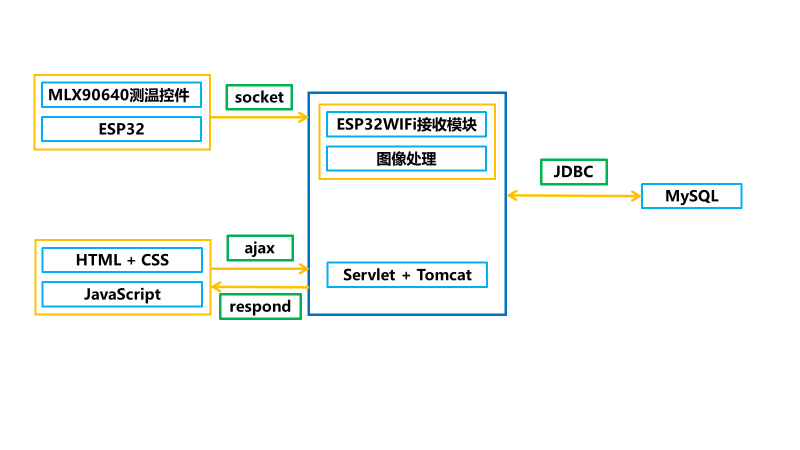
\includegraphics[width=0.8\textwidth]{design_1.png}
    \caption{总体设计}\label{fig:design_1}
    \vspace{\baselineskip}
    \end{figure}


\section{硬件系统设计}
(1)MLX90640温度采集模块

MLX90640 是工业标准并经过完全校准的 32*24
像素热红外阵列传感器,采用 4 脚 TO39 封装以及
I2C 兼容的数字接口。
MLX90640 包含 768 个热红外像素点。内嵌自身
环境温度传感器和 VDD 电压检测 ADC。通过 I2C 接
口,可以访问存储于内部 RAM 中的红外阵列、环境
温度以及 VDD 实时数据。

(2)ESP32模块
ESP32是一款安全稳定、低功耗、低成本的物联网芯片,搭载 RISC-V 32 位单核处理器,支持 2.4 GHz Wi-Fi 和 Bluetooth LE 5.0。为物联网产品提供行业领先的射频性能、完善的安全机制和丰富的内存资源。ESP32-C3 对 Wi-Fi 和 Bluetooth LE 5.0 的双重支持降低了设备配网难度,适用于广泛的物联网应用场景。


	\chapter{测试与开发过程}
\section{传播延时方面}
\begin{itemize}
    \item 最初方案:对float数组逐个传输,传完一次数据约耗时2s
    \item 改进方案:将float数组拼接为字符串,传完一次数据约耗时0.6s
    \item 尝试:使用udp进行传输,受包的大小限制,且不可靠传输导致顺序的错乱,放弃
    \item 最终方案:在ESP32上对float做乘100后类型转换为int,而后拼为字符串进行传输,降低了字符串的长度,传完一组数据约耗时0.3s
    \end{itemize}
\section{WiFi传输方案的选择}
\begin{itemize}
    \item 最初方案:使用ESP32开设热点,电脑连接进行数据发送。缺点:电脑不能上网
    \item 改进方案:使ESP32和电脑连接同一个局域网。缺点:每次更换网络环境,需要重新烧写。
    \item 第二次改进:先让ESP32开设热点,作为服务器提供一个html网页来输入网络名称和密码。缺点:每次启动都需要输入一次。
    \item 最终方案:保存上次连接的WiFi,启动后先尝试连接上次连接的WiFi,不成功再开启热点连接新的网络。
    \end{itemize}
\section{插值算法的选择}
\begin{itemize}
    \item 最初方案:简单的取平均值算法,精度不高,生成的图像比较模糊,细节缺失较多。
    \item 最终方案:实现了二元和三元插值算法,由于两种算法得到的图像差距较小,且二次插值算法在时间复杂度上有较大的优势,因此选择了二次插值算法。
    \end{itemize}
\section{温度区间色彩}
\begin{itemize}
    \item 最初方案:简单的让温度在色彩条带上均匀分布,由于温度跨度较大,而实际测温时的温度范围比较小,使得人和环境难以区分。
    \item 尝试:将温度低于一个值的颜色置为黑/白色,细节缺失较多,观感也不佳。
    \item 最终方案:根据实际情况,将人体体温附近的温度在色彩区间上占比增加,调整了其他温度区间的色彩区间占比,显著提升了成像的质量。
    \end{itemize}
\section{图片的产生和输出}
\begin{itemize}
    \item 最初方案:先在本地生成图片,再对本地生成的图片转为Base64编码。由于刷新速率快,每次运行产生大量图片。
    \item 最终方案:将生成的图片赋给一个image对象,直接对其进行Base64编码的转换。
    \end{itemize}
\section{服务器的部署}
    \begin{itemize}
    \item 最初方案:服务器部署于本机。缺点:必须通过局域网才能访问,硬件部分每次重新启动服务器也需要重新启动。
    \item 改进方案:将服务器部署在阿里云上,使得可以通过公网ip访问。
    \item 最终方案:设立两个服务器轮流运行,每次重启时连接另一个服务器并关闭前一个服务器进程,使得服务器可以一直运行,随用随连。
    \end{itemize}
\section{前端页面的改进}
\begin{itemize}
    \item 使得Web适配了电脑、手机、平板,真正实现了多端访问的需求。
    \end{itemize}

	\chapter{成果展示}
\begin{figure}[htbp]
    \centering
    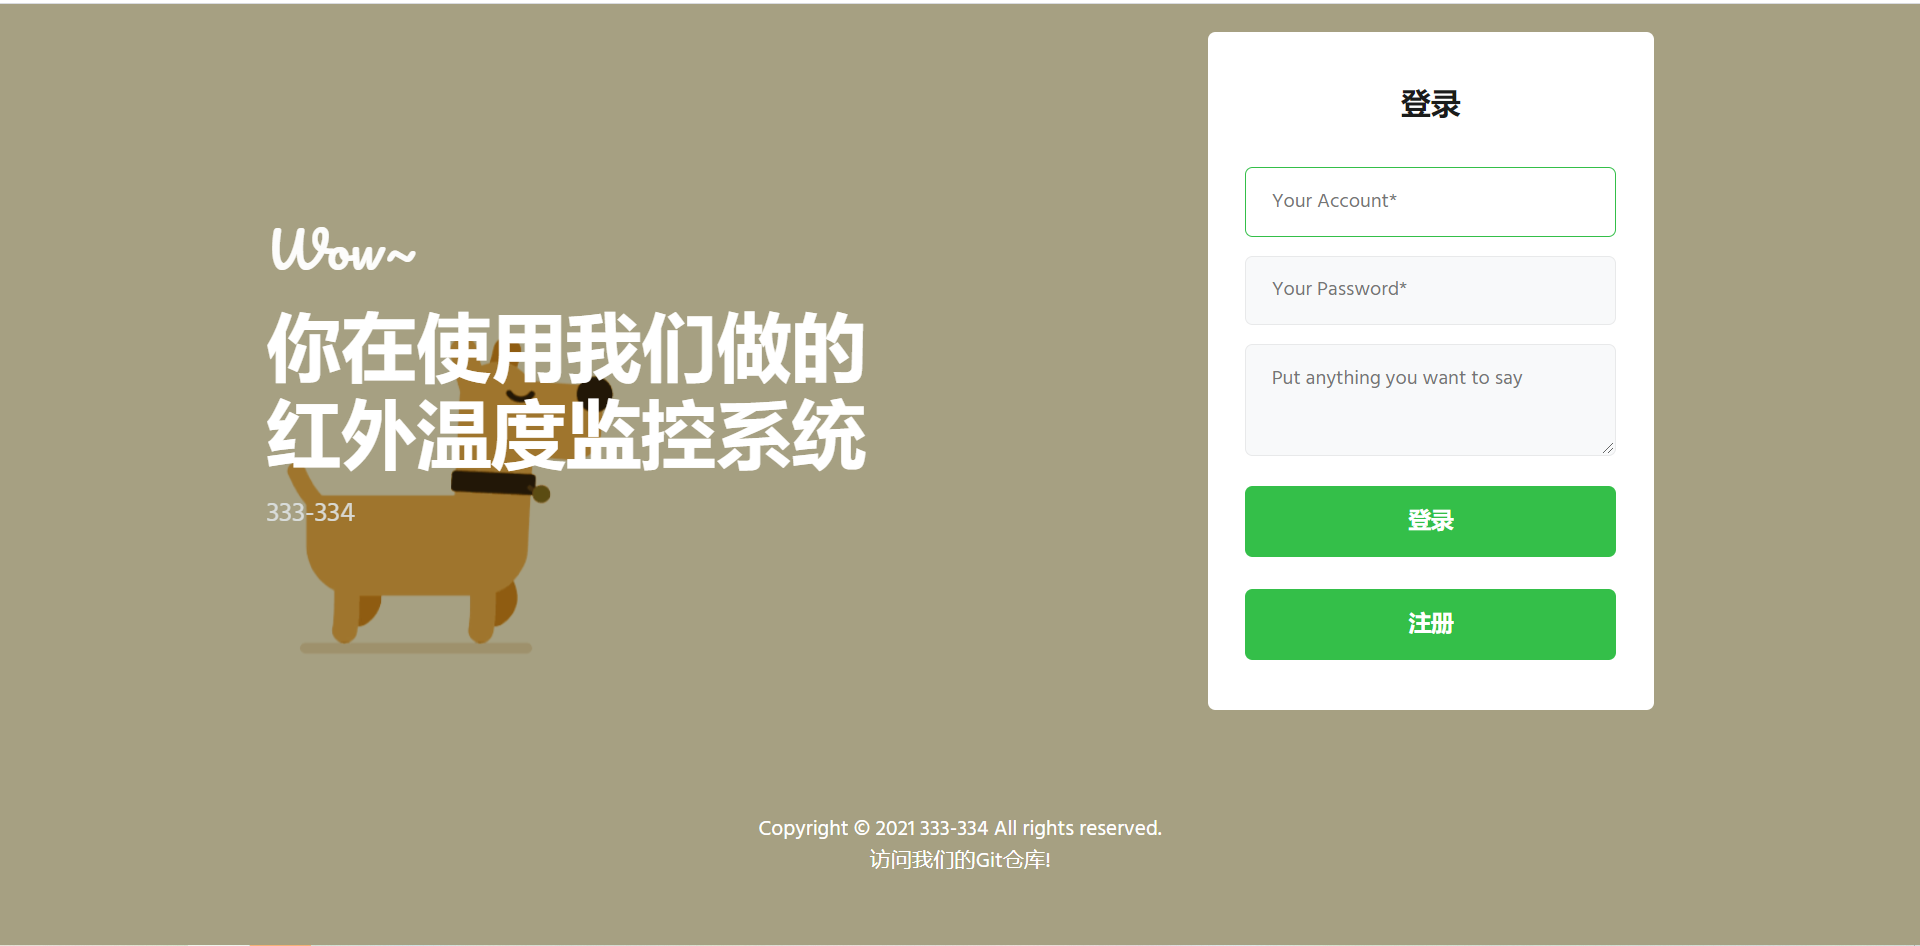
\includegraphics[width=1\textwidth]{show1.png}
    \caption{登录页面}\label{fig:show1}
    \vspace{\baselineskip}
    \end{figure}
    \begin{figure}[htbp]
        \centering
        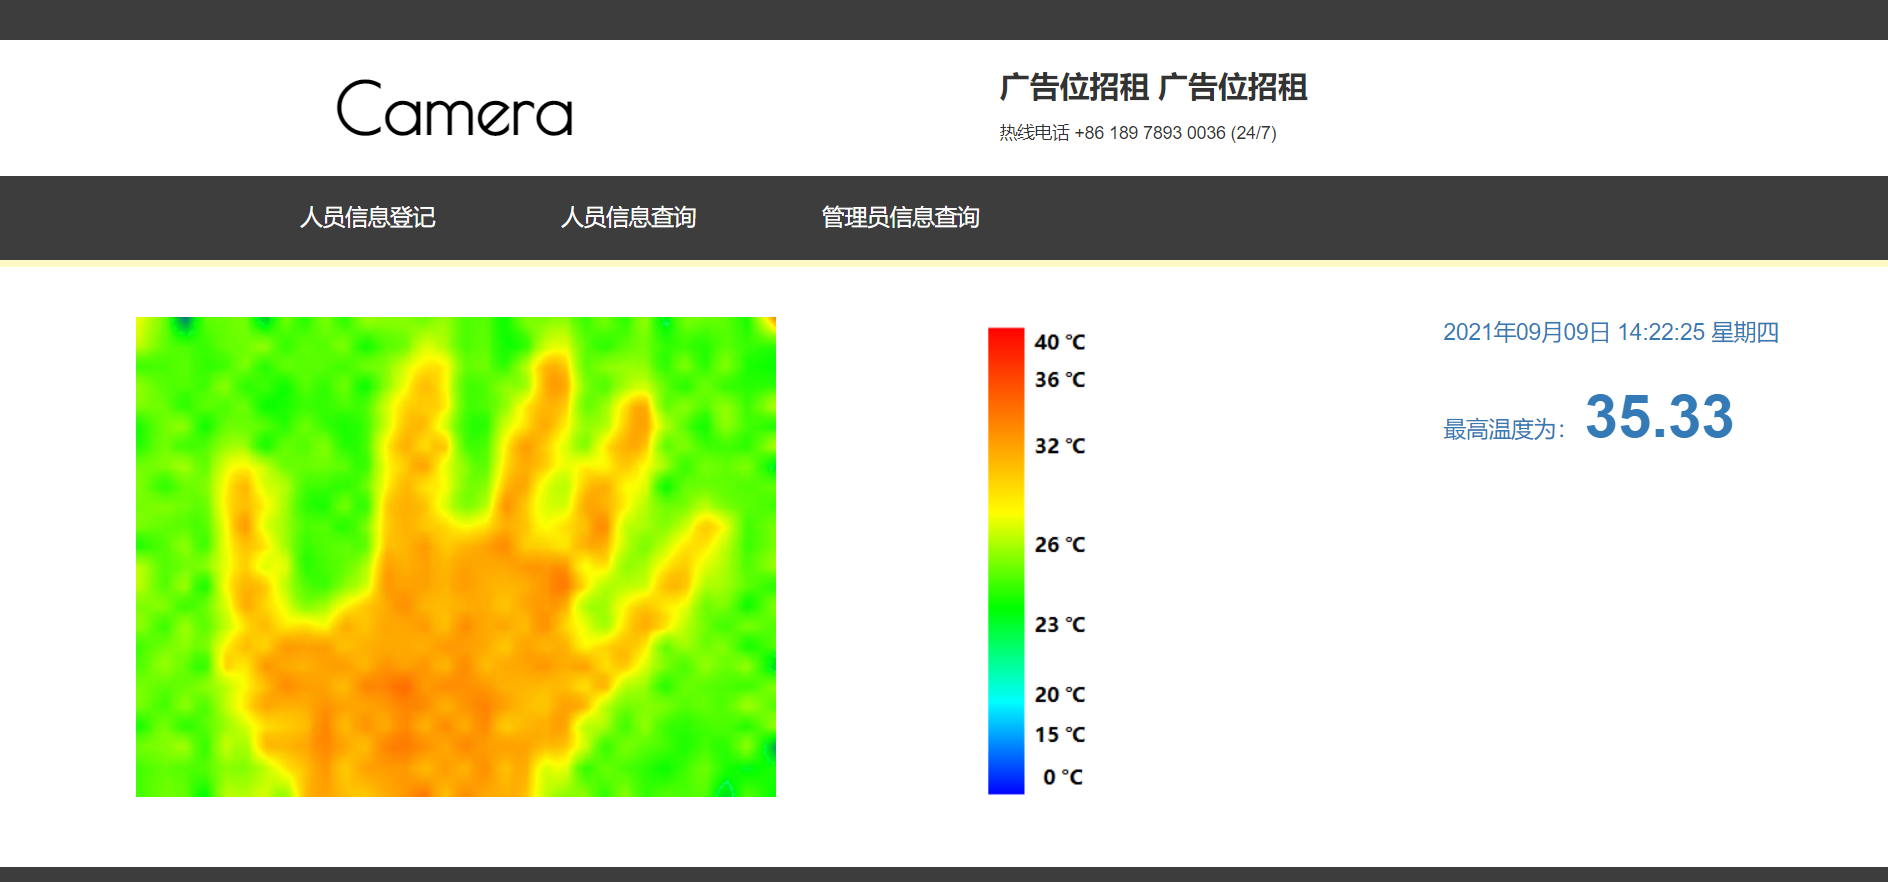
\includegraphics[width=1\textwidth]{show2.png}
        \caption{主界面}\label{fig:show2}
        \vspace{\baselineskip}
        \end{figure}
    \begin{figure}[htbp]
            \centering
            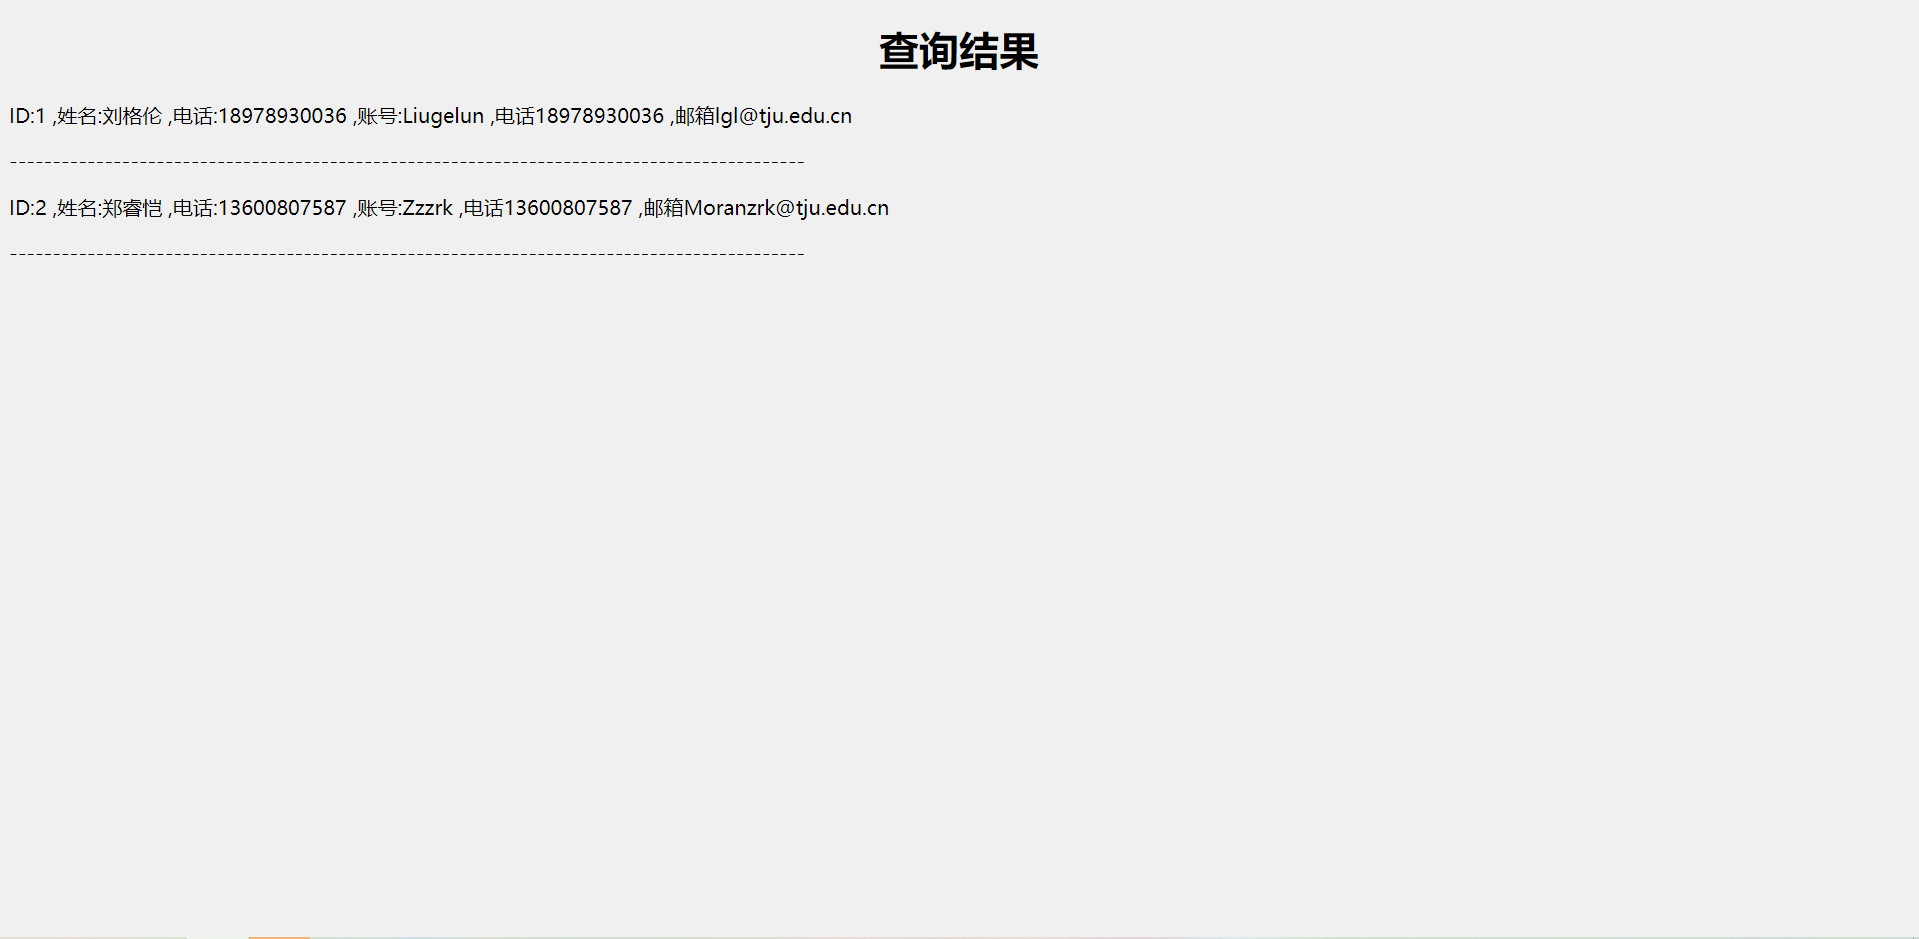
\includegraphics[width=1\textwidth]{show3.png}
            \caption{管理员信息查询}\label{fig:show3}
            \vspace{\baselineskip}
            \end{figure}
    \begin{figure}[htbp]
                \centering
                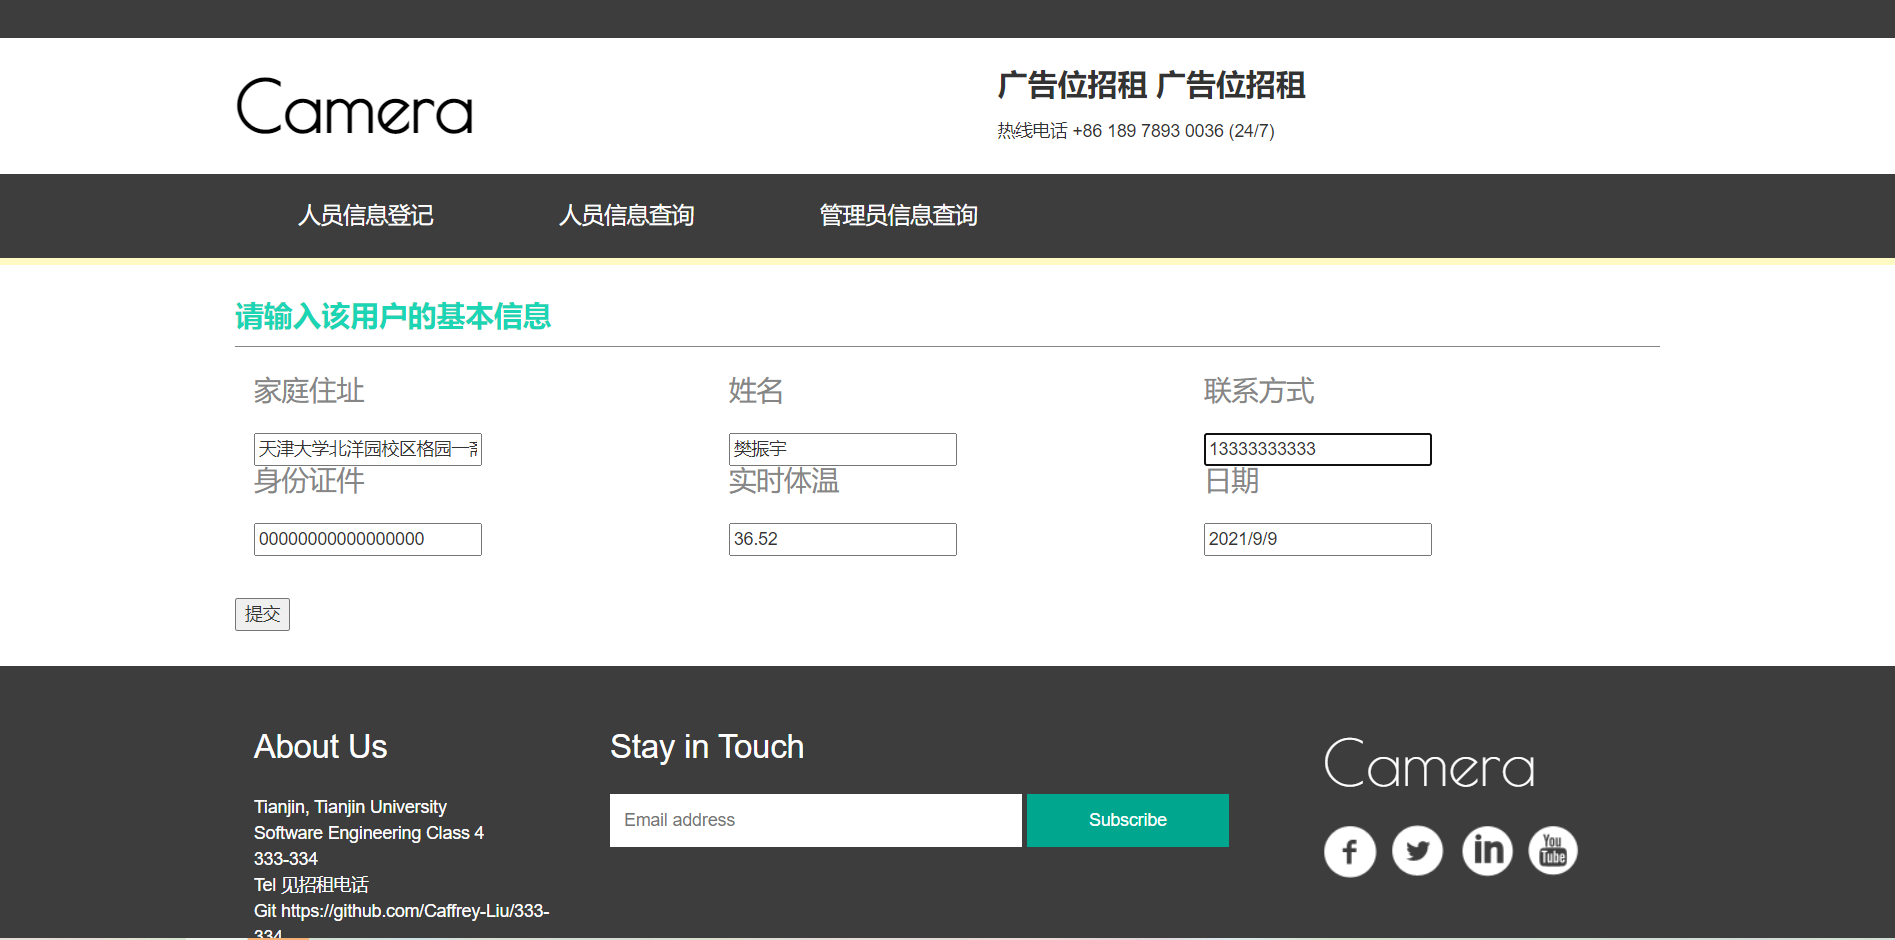
\includegraphics[width=1\textwidth]{show4.png}
                \caption{用户信息登记}\label{fig:show4}
                \vspace{\baselineskip}
                \end{figure}
                \begin{figure}[htbp]
                    \centering
                    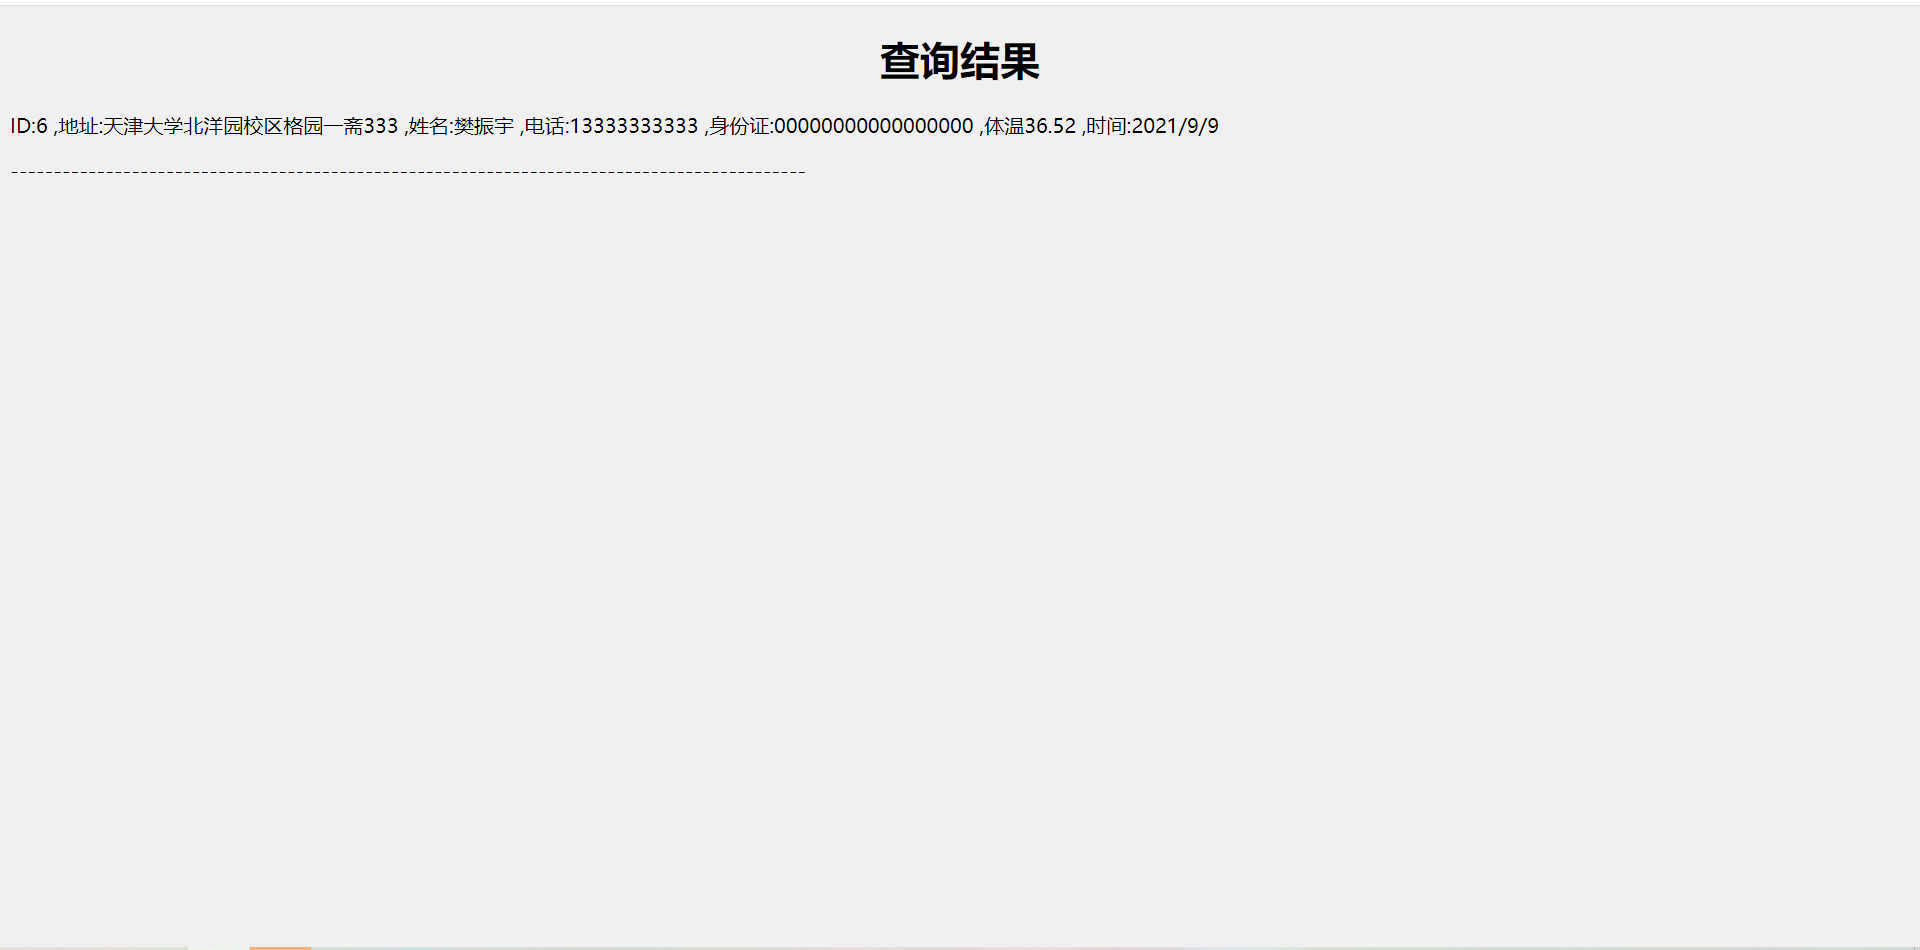
\includegraphics[width=0.8\textwidth]{show5.png}
                    \caption{用户信息查询}\label{fig:show5}
                    \vspace{\baselineskip}
                    \end{figure}
	\chapter{总结与展望}
\section{总结}
在本次实践中,我们实现了基于MLX90640传感器的Web平台开发,实现了基本的功能。对本次实践的全过程进行一个总结如下:
\begin{itemize}
    \item 由于缺乏项目的开发经验,起初进行开发时不知道从何入手。开始时没有明确的方向,各个模块都有所进展,却没有解决根本的前后端如何通信这样的问题。因此在前后端整合上花费了大量的时间。
    \item 通过这一次的开发过程,理解了如计算机网络,数据库这一类基础课程的重要性。在学习课本上理论知识的同时,将这些知识结合编程语言,结合到实际的项目中去,是学习这些课程必须要做到的。
    \item 总的来说,这次实践串联起之前所学的理论知识,并且让我们自己了解了许多实际项目中需要考虑的问题,收获颇丰。
    \end{itemize}
\section{展望}
本次实践基本实现了项目的需求,但目前还不够完善,存在可以拓展的功能,有以下几个想法:
\begin{itemize}
    \item 超过一定温度时,发出警报,如弹窗,发出声音等。
    \item 增加一个摄像头,进行人脸识别,实现来往人员信息的自动登记。
    \item 查询页面制作较为粗糙,有待改进。
    \end{itemize}
	\chapter{团队成员分工描述}

\underline{刘格伦}
\begin{itemize}
    \item 实现红外温度到可视颜色的伪彩色编码转换
    \item 建立服务器,对收到的数据进行处理
    \item 实现热成像图的绘制
    \item 实现前后端的通信
    \item 前端页面的美化
    \end{itemize}

\underline{郑睿恺}
\begin{itemize}
    \item 实现ESP32和红外传感器的数据采集方案
    \item 实现和改进ESP32的WiFi通信
    \item 实现二元和三元插值算法
    \item LaTex文档的编写
    \end{itemize}

\underline{樊振宇}
\begin{itemize}
    \item 数据库的建立,sql语句的编写
    \item 协助完成LaTeX文档的编写
    \end{itemize}
    
    \underline{周子涵}
\begin{itemize}
    \item 协助完成前端页面
    \item 协助完成LaTeX文档的编写
    \end{itemize}
    
    \underline{李世军}
\begin{itemize}
    \item 英文文献的翻译
    \end{itemize}









	\chapter{异构计算的uid及实验截图}
\begin{figure}[htbp]
    \centering
    \includegraphics[width=0.4\textwidth]{文件名(.eps)}
    \caption{标题}\label{标签名(通常为 fig:labelname)}
    \vspace{\baselineskip} % 表示图与正文空一行
    \end{figure}


	% \clearpage

\end{CJK*}                                     % 结束中文字体使用
\end{document}                                 % 结束全文
